\chapter{Umsetzung}

Nachdem die Ziele der angestrebten TypeScript-Migration charakterisiert und die Anforderungen an den geplanten Transpiler ausgeführt wurden, soll im Folgenden der Entwurf und die Details der entsprechend gewählten Implementierung ausgeführt werden.
In Abschnitt~\ref{subsec:js-transpilers} wurden bereits die verbreitetsten Werkzeuge im Umfeld der Transpilierung von JavaScript ausführlich vorgestellt und verglichen. Auf Basis dieser Gegenüberstellung wurde schließlich Babel~\autocite{BABEL} als Grundlage der vorliegenden Implementierung des Transpilers von Flow nach TypeScript gewählt.

% CITATION NEEDED
Im Gegensatz zu den betrachteten Alternativen unterstützt lediglich Babel die Syntax von Flow, TypeScript und moderner bzw. experimenteller JavaScript-Sprachkonstrukte vollständig. Dieser Aspekt ist entscheidend, da nur so eine universelle Übersetzung \emph{jeglicher} Flow-Syntax in äquivalentes TypeScript umgesetzt werden kann\footnote{vgl. Anforderung~\ref{subsection:requirement:correct-translation}}. Ein weiteres Argument für die Wahl von Babel ist einerseits die sehr gute Erweiterbarkeit durch ein Plugin-System, andererseits die Ausgereiftheit und große Verbreitung des Projekts. Keine der anderen Optionen konnte die Anforderungen des Transpilers in vergleichbarem Maße erfüllen.

\section{Software-Architektur}

\subsection{Funktionsweise von Babel-Plugins}

Zur Erleichterung des Verständnisses der weiteren Ausführung der Implementierung soll zunächst ein Überblick über die Funktionsweise von Babel-Plugins gegeben werden. Der Kern von Babel selbst setzt sich aus einer Vielzahl von Plugins zusammen, welche in ihrer Gesamtheit die Funktionalität des Compilers realisieren~\autocite{BABEL}. Dies verdeutlicht die tiefgreifend integrierte Modularität des Systems. Plugins sind die elementaren Bausteine, die eine flexible Erweiterung des Compilers um neue Funktionen ermöglichen.
Mit der Entscheidung den Flow-Transpiler als Babel-Plugin umzusetzen, ist dessen Grundarchitektur bereits in Teilen festgelegt, da alle Plugins die vorgegebenen Programmschnittstellen von Babel implementieren müssen. Der konzeptionelle Ablauf eines Plugins gliedert sich in folgende drei Phasen~\autocite{BABEL_HANDBOOK}:

% TODO: Tokenizer, Lexer, Tokens und all den Quatsch in den Grundlagen erklären!
\begin{enumerate}
  \item \textbf{Parsen des Eingabecodes}

    Zunächst wird der ursprüngliche Quelltext in zwei Schritten eingelesen, um den abstrakten Syntaxbaum (AST) des Programms zu erzeugen: Als Erstes wird der Code während der lexikalischen Analyse mittels des Tokenizers in Tokens zerlegt. Anschließend werden diese in der syntaktischen Analyse zu einer Datenstruktur umgeformt, die den zugehörigen Syntaxbaum repräsentiert.
    \\

  \item \textbf{Transformation des Programms}

    Während der zweiten Phase wird daraufhin die eigentliche Programmtransformation durchgeführt: Dabei wird der abstrakte Syntaxbaum mittels des \textit{Besucher}"=Entwurfsmusters rekursiv traversiert und die Knoten des Baums sukzessive modifiziert, gelöscht bzw. neu erstellte Elemente eingefügt~\autocite{BABEL_HANDBOOK}. Das Besucher-Entwurfsmuster\footnote{Dieses Entwurfsmuster (engl. \textit{Visitor-Pattern.}) gehört zu den 23 Entwurfsmustern, die im Standardwerk \citetitle{GAMMA:1994} der \enquote{Gang of Four} (E. Gamma, R. Helm, R. Johnson und J. Vlissides) beschrieben werden~\autocite[306\psqq]{GAMMA:1994}.} beschreibt, wie Operationen auf einer Objektdatenstruktur, unabhängig von der konkreten Implementierung der zugrunde liegenden Klassen, durchgeführt werden können~\autocite[634\psq]{Freeman:2004}. Im vorliegenden Fall ermöglicht die Anwendung des Musters die gewünschte Menge der Knoten des Syntaxbaums individuell zu \enquote{besuchen} und dort die gewünschte Transformation des Programms umzusetzen.
    \\

  \item \textbf{Generierung des Ausgabequelltexts}

    Schließlich kann der Ausgabecode generiert werden: Hierbei werden alle Knoten des abstrakten Syntaxbaums durch Anwendung einer Tiefensuche nach und nach durchlaufen und eine Zeichenkette aufgebaut, welche den modifizierten, endgültigen Quelltext darstellt.
\end{enumerate}

Im Folgenden wird das Hauptaugenmerk der Betrachtung auf die zweite Phase gelegt, da hier die Lösung der vorliegenden Problemstellung, die Transpilierung von Flow- nach TypeScript, realisiert wird. Das Parsen der Eingabe und das Generieren der Ausgabe kann durch Verwendung der gegebenen Standard-Funktionen von Babel simpel umgesetzt werden.

\subsection{Konzeptioneller Aufbau des Transpilers}

Abbildung~\ref{fig:activity-diagram-transpiler} auf Seite~\pageref{fig:activity-diagram-transpiler} zeigt das Aktivitätsdiagramm\footnote{Aktivitätsdiagramme (engl. \textit{activity diagram}) entstammen der Modellierungssprache \textit{Unified Modeling Language} (UML) und TODO.} der umgesetzten Implementierung als Babel-Plugin.

\begin{figure}[p]
  \centering
  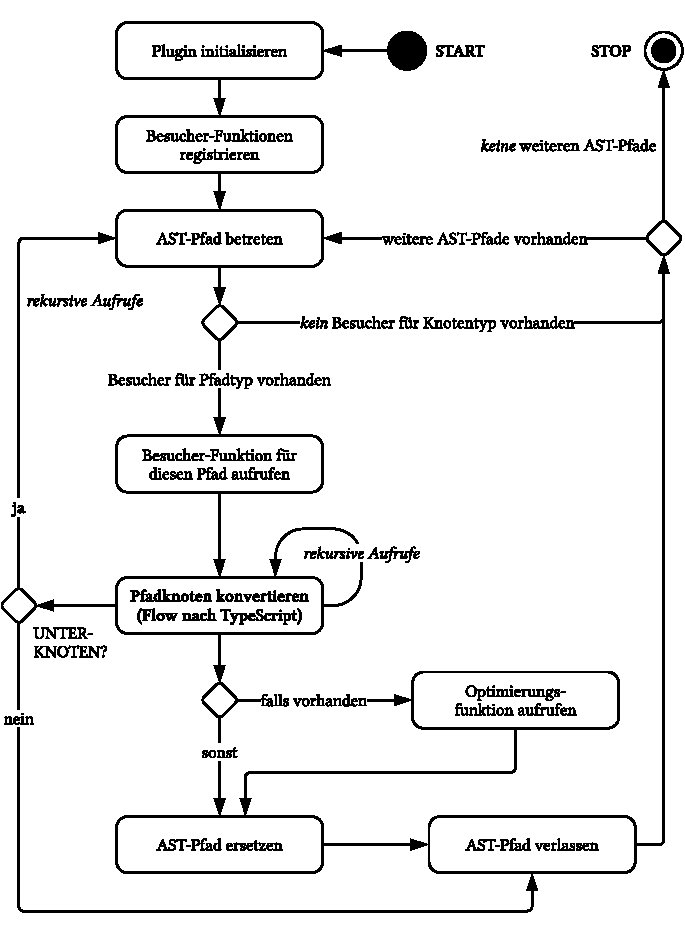
\includegraphics[width=0.84\textwidth]{src/4_Umsetzung/img/activity-diagram-transpiler.pdf}
  \captionsetup{justification=centering}
  \caption{Aktivitätsdiagramm des Transpilers (Babel-Plugin).}
  \label{fig:activity-diagram-transpiler}
\end{figure}

\section{Entwicklungsprozess}

\subsection{Testgetriebene Entwicklung}

Die korrekte Übersetzung der Flow-Typen ist die wichtigste Anforderung an den Transpiler. Essentiell ist daher die Bereitstellung zuverlässiger Testmechanismen, um Regressionen während der Entwicklungphase frühzeitig festzustellen. Zur Gewährleistung dieser Anforderung wurde der Ansatz der \enquote{testgetriebenen Entwicklung}\footnote{engl. \textit{Test-driven development (TDD).}} gewählt, um die korrekte Funktionalität und Wechselwirkung aller Bestandteile des Transpilers kontinuierlich zu überprüfen. Die testgetriebene Entwicklung hat ihren Ursprung im Vorgehensmodell \enquote{Extreme Programming}~\autocite{JEFFRIES:EXTREME_PROGRAMMING} aus der Software-Entwicklung und sieht im Gegensatz zu klassischen, seriellen Vorgehensweisen wie dem Wasserfall-Modell vor, dass alle Testfälle eines Features bereits \emph{vor} dessen Umsetzung geschrieben werden müssen~\autocite{KENT:EXTREME_PROGRAMMING}. Die Vorteile dieser Methodik ist die Sicherstellung einer hohen Testabdeckung und die Erzielung einer Implementierung, welche die Anforderungen \emph{vollständig} erfüllt, sofern die Testfälle sorgfältig spezifiziert wurden.



% Verlagerung des Fokus auf die korrekte Erfüllung der Software-Anforderungen, indem diese .

% Hierdurch wird sicher gestellt, dass der Programmierer sich \emph{zuerst} Gedanken über die konkrete Eingabe und erwartete Ausgabe einer Funktion machen muss und erst danach mit der Umsetzung beginnt.

% da auf diese Weise sichergestellt wird, dass eine hohe Testabdeckung der Transformationsroutinen besteht.

% Irgendwo sollte wohl geschrieben werden, dass TypeScript, TDD usw. verwendet wurde, um das Plugin zu bauen\dots

\section{Implementierung als Babel-Plugin}
  \subsection{Transpilierung der Basistypen}
  \subsection{Transpilierung der Hilfstypen}
  \subsection{Transpilierung der Deklarationen}

  \subsection{Weitere Optimierungen}
    \subsubsection{Übersetzung gängiger Typimporte}
    \subsubsection{Konvertierung von Class Decorators}

  Mapping der Importe (verschiedene Typnamen in Flow und TS), Umwandlung der Decorators usw.

\section{Erweiterung als Kommandozeilenprogramm}

Aufgrund der in Abschnitt~\ref{subsection:requirement:batch-processing} dargelegten Anforderung, dass der Transpiler in der Lage sein muss gesamte Projektverzeichnisse zu verarbeiten, ist eine Erweiterung als Kommandozeilenprogramm naheliegend. Hierdurch können beliebige Dateien und Verzeichnisse eingelesen und übersetzt werden.

% Dieses nimmt einzelne Eingabedateien oder -verzeichnisse als Argument entgegen und besitzt weiterhin verschiedene Optionen, um den Transpilierungsvorgang

Abbildung~\ref{fig:activity-diagram-transpiler-cli} auf Seite~\pageref{fig:activity-diagram-transpiler-cli} zeigt das Aktivitätsdiagramm der Anwendung.
% Dieses stellt lediglich eine schmale Ummantelung des Babel-Plugins dar
% Dieses bietet diverse Optionen, welche dem Benutzer ermöglichen die Transpilierung

\begin{figure}[p]
  \centering
  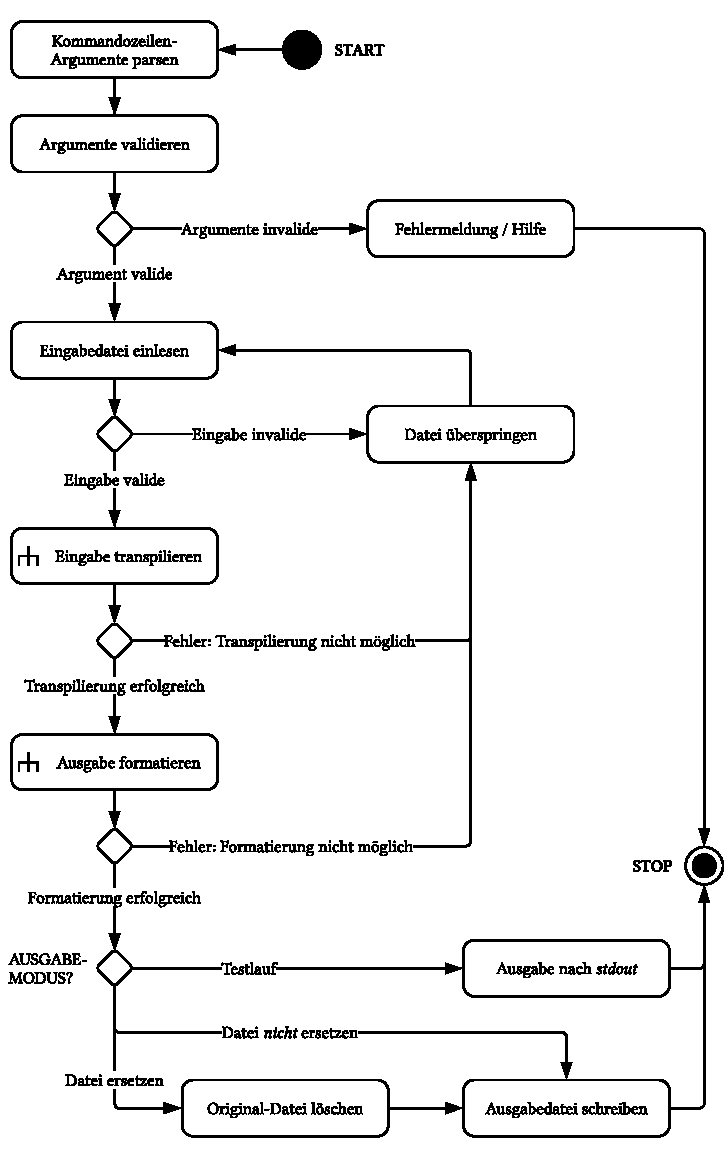
\includegraphics[width=0.84\textwidth]{src/4_Umsetzung/img/activity-diagram-transpiler-cli.pdf}
	\caption[Aktivitätsdiagramm des Kommandozeilenprogramms]{Aktivitätsdiagramm des Kommandozeilenprogramms. Vgl. eingebettete Diagramme~\ref{fig:activity-diagram-transpiler} \enquote{Eingabe transpilieren} und~\ref{fig:activity-diagram-formatting} \enquote{Ausgabe formatieren}.}
	\label{fig:activity-diagram-transpiler-cli}
\end{figure}

\section{Formatierung des Ausgabequelltexts}

\begin{figure}[htbp]
  \centering
  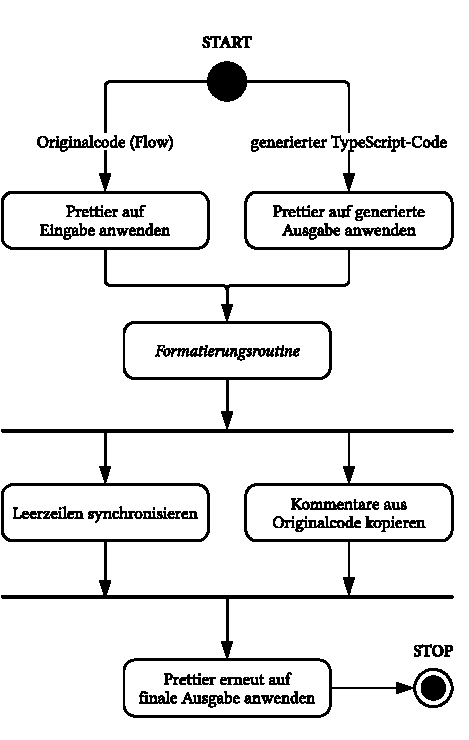
\includegraphics[width=0.6\textwidth]{src/4_Umsetzung/img/activity-diagram-formatting.pdf}
  \captionsetup{justification=centering}
	\caption[Aktivitätsdiagramm der Formatierung des Ausgabecodes]{Aktivitätsdiagramm der Formatierung des generierten Ausgabecodes.}
	\label{fig:activity-diagram-formatting}
\end{figure}

Prettier, synchronisieren der Leerzeilen und Kommentare beschreiben usw.
